\chapter{Convección Mixta En Transición Laminar-Turbulenta} \label{cap:transicion}

En el presente capítulo se examina la transición laminar-turbulenta en convección mixta en un canal de placas paralelas mediante simulaciones DNS. El mismo se organiza en tres partes: (i) la exploración de distintas condiciones iniciales mediante la evolución temporal de magnitudes de interés (TKE y Re$_{\tau}$) contemplando dos valores del número de Richardson Ri$_b$ (casos A y B); (ii) un análisis detallado del caso correspondiente al Ri$_b$ más bajo simulado (ensayo A-C10); (iii) un análisis detallado del caso correspondiente al Ri$_b$ más alto simulado (ensayo B-C2).

En los ensayos A-C10 y B-C2 se consideran las siguientes magnitudes de interés: la energía cinética turbulenta (TKE) y la varianza de la temperatura adimensional; perfiles de velocidad y de temperatura adimensional en instantes representativos; el factor de fricción de Darcy y número de Nusselt. Este conjunto de métricas permite vincular la dinámica de la transición con su impacto termo-hidrodinámico y con el acercamiento a los estados de referencia completamente desarrollados.

En los ensayos con Ri$_b$ más bajo ($\text{Ri}_b=0\text{.}04$) se requirió emplear una combinación de perturbaciones bidimensionales y tridimensionales para desencadenar la transición. Por su parte, aquellos ensayos con Ri$_b$ más alto ($\text{Ri}_b=1\text{.}06$), si bien también se consideraron condiciones iniciales construidas con combinaciones de ondas 2D/3D, fue posible inestabilizar el flujo empleando únicamente ondas 2D. 

En el ensayo A-C10, en una etapa inicial ($t^*\lesssim 400$), la evolución temporal de las \linebreak cantidades se caracteriza por experimentar mínimos y/o máximos locales y absolutos, \linebreak salvo en el número de Nusselt que en esta etapa se mantiene prácticamente constante. Luego, estas magnitudes tienden hacia el estado turbulento desarrollado. En particular, las cantidades asociadas al campo hidrodinámico del sistema evolucionan a mayor ritmo respecto de aquellas cantidades asociadas al campo térmico. Al inspeccionar los perfiles de velocidad y temperatura es posible apreciar una pérdida de simetría. Mediante un análisis cualitativo de las estructuras de vórtices, es posible visualizar que las mismas se aglomeran de manera no uniforme cerca de las paredes dando cierto entendimiento a esta última cuestión.  

Por otro lado, en el ensayo B-C2, las magnitudes de interés experimentan un breve período laminar y luego tienen un crecimiento brusco, salvo el número de Nusselt que decrece. Esta cuestión ocurre en los instantes de tiempo tales que $t^*\lesssim 50$. El decrecimiento de Nu está ligado a un aumento de la energía cinética turbulenta producto del crecimiento de la turbulencia en el flujo. Para tiempos posteriores, luego de experimentar esa subida, las cantidades decrecen y tienden hacia el estado turbulento desarrollado con la excepción de Nu que tiende a recupersarse de su mínimo. Si bien Nu alcanza y supera el valor del estado inicial, en la ventana de tiempo simulada, la magnitud no alcanza el valor de referencia del estado desarrollado. 

Por último, se comparan similitudes y diferencias entre los ensayos A-C10 y B-C2. En particular, se compara la evolución temporal del Reynolds de fricción (Re$_{\tau}$). En el ensayo \linebreak A-C10 el estado final queda por encima del valor inicial mientras que en B-C2 queda por debajo. Esta diferencia entre ambos puede explicarse como un efecto del aumento de la turbulencia en el flujo (medida en términos de la energía cinética turbulenta) que influye sobre los perfiles de velocidad.


\section{Exploración de casos} \label{sec:explo}

Como se menciona en los Capítulos \ref{cap:intro} y \ref{cap:modelo}, la convección mixta en canales ha sido investigada exhaustivamente debido a sus múltiples aplicaciones de interés. Sin embargo, la transición laminar-turbulenta en convección mixta es un fenómeno que no ha sido estudiado en profundidad. En la bibliografía reciente existen escasos trabajos, uno de ellos es el de Chen y Chung \cite{chen2003direct}, donde se analiza el fenómeno de transición temporal.

Por esta razón, se realiza primero una exploración numérica que permita identificar combinaciones de perturbaciones capaces de inducir la inestabilidad del flujo. Se seleccionan dos números de Richardson \textit{bulk} que corresponden a soluciones desarrolladas con diferentes \linebreak características: una levemente afectada por la fuerza boyante y la otra con perfiles de velocidad y temperatura claramente influidos por la flotación. Estos corresponden a los casos A y B de la Tabla \ref{tab:cases}, respectivamente, y en ambos se considera Re$_o$=5000 y Pr=0.71.

El mecanismo de inestabilización se construye a partir de condiciones iniciales de acuerdo con las ecuaciones \ref{eq:init_con_1} - \ref{eq:init_con_3} seleccionando distintos números de onda y amplitudes (véase Sección \ref{sec:mecanismo}). Los autovalores y sus autofunciones asociadas se obtuvieron mediante el análisis de estabilidad lineal descrito en el Capítulo \ref{cap:modelo}, utilizando la herramienta OSMC descrita en el Capítulo \ref{cap:numerico}. El espectro de autovalores y las autofunciones utilizadas en este trabajo pueden consultarse en el Apéndice \ref{cap:transition_apendice}. 

Por otro lado, para decidir si una perturbación arbitraria es capaz de inestabilizar el flujo se estudia la evolución temporal de las siguientes magnitudes:

\begin{itemize}
  \item la energía cinética turbulenta, TKE o $\kappa$, definida en el Capítulo \ref{cap:modelo},
  	\begin{equation*}
  		\text{TKE} = \frac{1}{2} \left[ \langle u^{* \prime}_x u^{* \prime}_x \rangle + \langle u^{* \prime}_y u^{* \prime}_y \rangle + \langle u^{* \prime}_z u^{* \prime}_z \rangle \right] ; 
  	\end{equation*}
  	
  

  \item y el número de Reynolds de fricción
        $$
          \text{Re}_{\tau} = \frac{u_{\tau}\,d}{\nu} , \quad u_{\tau}= U_o \sqrt{ \frac{1}{\text{Re}_o} \left. \frac{d \langle u^*_x \rangle}{dy^*} \right\vert_w }
        $$
        donde $u_{\tau}$ es la velocidad de fricción \cite{pope2001turbulent}.
\end{itemize}

\begin{table}[H]
\centering
\resizebox{0.24\textwidth}{!}{%
\begin{tabular}{lccc}
\toprule
Caso & Ri$_b$ & Ra \\
\midrule
A & 0.04 & 65 \\
B & 1.06 & 1775 \\
\bottomrule
\end{tabular}}
\caption{Parámetros adimensionales de los dos casos elegidos.}
\label{tab:cases}
\end{table}

\textit{\textbf{Aclaración Importante.}} En las siguientes secciones, el lector hallará gráficas con la evolución temporal de las magnitudes  Re$_{\tau}$, TKE, varianza de la temperatura, número de Nusselt (Nu) y factor de fricción de Darcy ($f$). En ellas, aparecen representados valores \linebreak constantes mediante líneas a trazos cuyas etiquetas contienen los subíndices ``Init'' y ``Dev''. El primer subíndice corresponde al cálculo de las magnitudes antes mencionadas empleando los perfiles de las condiciones iniciales ($t^*=0$); el segundo corresponde al cálculo de las magnitudes empleando los perfiles del flujo turbulento completamente desarrollado, presentados en el Capítulo \ref{cap:desarrollado}. Para el cálculo de Nu y $f$ se emplean las ecuaciones \ref{eq:nu} y \ref{eq:darcy}, respectivamente.

Los perfiles de velocidad y temperatura en $t^*=0$ son muy similares a los perfiles del flujo base laminar.  Por lo cual, los valores de Re$_{\tau}$, Nu y $f$ calculados con la condición inicial son equivalentes a los calculados en el régimen laminar. Asimismo, los valores de TKE y la varianza de la temperatura se aproximan utilizando las autofunciones $\lbrace \widehat{v_x}, \widehat{v_y}, \widehat{v_z}, \widehat{\theta} \hspace{0.3mm} \rbrace$ que aparecen en las expresiones de las perturbaciones. Esto surge de considerar lo siguiente: 

$$\xi^{\prime} (x^*,y^*,z^*,t^* = 0) \equiv \widetilde{\xi}(x^*,y^*,z^*,t^*=0) =  \widehat{\xi}(y^*) e^{i (\alpha x^* + \beta z^*)} , $$
donde $\widetilde{\xi}$ representa una perturbación arbitraria y $\widehat{\xi}$ su amplitud asociada. De esta manera, en $t^*=0$, los valores de TKE y $\langle \theta^{* \prime} \theta^{* \prime} \rangle$ se estiman mediante las relaciones \ref{eq:tke-calc} y \ref{eq:varteta-calc} donde $\widetilde{\mathbf{v}}$ y $\widetilde{\varphi}$ están dadas por las ecuaciones \ref{eq:init_con_2} y \ref{eq:init_con_3}, respectivamente.

\begin{align}
\text{TKE}_{\text{Init}} &\equiv \frac{1}{2} \int \left[ \widetilde{\mathbf{v}} \cdot \widetilde{\mathbf{v}} \right] dx^* dy^* dz^* 
\label{eq:tke-calc}\\
\langle \theta^{* \prime} \theta^{* \prime} \rangle_{\text{Init}}  &\equiv \int \left[ \widetilde{\varphi} \hspace{0.2mm} \right]^2 dx^* dy^* dz^* 
\label{eq:varteta-calc}
\end{align}  

\newpage

\subsection{Caso A (Ri$_b$=0.04)}

En la Figura \ref{fig:case-A-Re5000-Pr071} se expone la evolución en el tiempo de TKE y Re$_{\tau}$ para las distintas condiciones iniciales consideradas. Los parámetros asociados a las perturbaciones de dichas condiciones se resumen en la Tabla \ref{tab:grupo1}. Adicionalmente, se añaden los valores asociados al caso turbulento completamente desarrollado (línea a trazos roja).  

Las condiciones iniciales de los cuatro primeros ensayos, de A‑C1 a A‑C4, se construyen empleando únicamente una onda bidimensional y un mismo conjunto de autofunciones cuya parte imaginaria del autovalor ($c_{2D}$=1.212 + 0.037 j) es la cota superior\footnote{Esto  se conoce como modo más inestable \cite{schmid}.} de todo el espectro de autovalores asociado. En estos ensayos sólo se varía la amplitud de las perturbaciones 2D de 1 \% a 6 \% (Tabla \ref{tab:grupo1}). Se observa que, en el tiempo simulado, no se logra inducir la transición del flujo. En su lugar, el efecto que se logra es la traslación (adelanto) del máximo en la TKE desde $t^* \approx 140$ hasta $t^* \approx 80$. En todos los casos, luego de crecer y alcanzar un valor máximo, la TKE retorna a niveles próximos a cero. Por su parte, los valores de Re$_{\tau}$ permanecen practicamente constantes hasta $t^* \approx 100$ donde comienza un descenso de la magnitud (un total de aprox 8 \%) y posteriormente tiende a recuperarse y evolucionar, aparentemente, hacia su estado inicial, más allá del intervalo temporal simulado. Como lo que se busca es una transición temprana del flujo, y además, como no se observa una estabilización no nula en la TKE, se opta por finalizar las simulaciones de estos ensayos.  

Por otro lado, se trata de inducir la inestabilidad empleando otras autofunciones. Se conserva la amplitud (6 \%) y se utilizan autofunciones de modos menos inestables (véase Tabla \ref{tab:grupo1} y Apéndice \ref{cap:transition_apendice}). Estos casos corresponden a los ensayos A-C7 y A-C8. En ambos, la TKE crece hasta un máximo absoluto, que continúa con un segundo máximo local de menor intensidad y finaliza con una pequeña réplica de aún menor intensidad (aproximadamente un orden de magnitud menor) para luego retornar a valores próximos al estado inicial. El comportamiento descrito es similar en ambos casos, con la diferencia que en el ensayo A-C7 la dinámica se retrasa respecto a la de A-C8. Esta cuestión coincide con el hecho de que la parte imaginaria del autovalor correspondiente a A-C7 es mayor que la de A-C8. El retraso en la dinámica se aprecia al comparar ambos máximos absolutos: para A-C7 el máximo se encuentra en $t^* \approx 340$, mientras que para A-C8 está ubicado en  $t^* \approx 180$. Por su parte, el descenso de Re$_{\tau}$ se retrasa en ambos casos, siendo más extenso en el ensayo A-C7. Luego, en los dos ensayos, el sistema adquiere una nueva condición de flujo que, al menos hasta el tiempo simulado, es distinta del estado inicial. No obstante, no se han encontrado indicios de que una transición temporal temprana vaya a ocurrir.  

El uso exclusivo de ondas bidimensionales resulta, aparentemente, insuficiente para desencadenar la transición del flujo. Por ello, resulta necesario buscar otra estrategia o herramienta que nos permita inestabilizar al mismo. Se procede entonces a emplear una combinación de \linebreak ondas bidimensionales y tridimensionales para construir una perturbación que pueda reproducir la inestabilidad secundaria (Sección \ref{sec:mecanismo}). En este sentido, las condiciones iniciales de los \linebreak ensayos A‑C9 y A‑C10 se construyen empleando la combinación de una onda 2D \linebreak (A$_\text{2D}=6$ \% y mismas autofunciones de los casos A-C7 y A-C8, respectivamente) con dos ondas 3D oblicuas (A$_\text{3D}=1$ \%). 

En una primera etapa, tanto la energía cinética turbulenta como el Re$_{\tau}$ reproducen el mismo comportamiento que experimentan los ensayos A‑C7 y A‑C8. Posteriormente, para $t^* \gtrsim 395$ (A-C9) y $t^* \gtrsim 240$ (A-C10), los casos se despegan y experimentan un crecimiento \linebreak brusco seguido de un pico y un ligero descenso. Luego, las magnitudes se sostienen en el tiempo en torno al valor del caso completamente desarrollado; es decir, no decaen como en los casos anteriores. Esto indica que la combinación de ondas 2D y 3D resulta exitosa para inestabilizar el flujo desde un régimen laminar hacia uno turbulento. Es destacable la utilidad del concepto de inestabilidad secundaria en estos ensayos. Este puede interpretarse de la siguiente forma: la perturbación 2D evoluciona a un nuevo estado pseudo-estacionario que persiste durante una ventana temporal y puede, posteriormente, interactuar constructivamente con la perturbación 3D y desencadenar la transición a la turbulencia.


\paragraph{Caso representativo.} El ensayo \textbf{A‑C10} se elige como referencia para la discusión \linebreak detallada (Sección \ref{sec:ac10}) ya que se logra una transición temprana del flujo ($t^* \approx 240$) que fue claramente inducida y además que se sostiene en el tiempo ($t^*>400$). 

\begin{table}[H]
\centering
\caption{Parámetros de las condiciones iniciales para el caso A (Re$_o$ = 5000, Pr = 0.71, Ri$_b$ = 0.04).}
\resizebox{0.8\textwidth}{!}{%
\begin{tabular}{lcccccc}
\toprule
Nomenclatura & $\alpha$ &   $\beta$ &   A$_{2D}$ [\%] &  A$_{3D}$ [\%] & $c_{2D}$ & $c_{3D}$ \\
\midrule
A-C1 &  1.12 & 0    & 1  & 0    & 1.212 + 0.037 j & - \\
A-C2 &  1.12 & 0    & 2  & 0    & 1.212 + 0.037 j & - \\
A-C3 &  1.12 & 0    & 4  & 0    & 1.212 + 0.037 j & - \\
A-C4 &  1.12 & 0    & 6  & 0    & 1.212 + 0.037 j & - \\
A-C7 &  1.12 & 0    & 6  & 0    & 0.472 - 0.104 j & - \\
A-C8 &  1.12 & 0    & 6  & 0    & 0.385 - 0.124 j & - \\
A-C9 &  1.12 & 2.1  & 6  & 1    & 0.472 - 0.104 j & 0.575 - 0.095 j \\
A-C10 & 1.12 & 2.1  & 6  & 1    & 0.385 - 0.124 j & 0.563 - 0.095 j \\
\bottomrule
\end{tabular}}
\label{tab:grupo1}
\end{table}

\newpage

\begin{figure}[H]
  \centering
  \subfloat[]{
    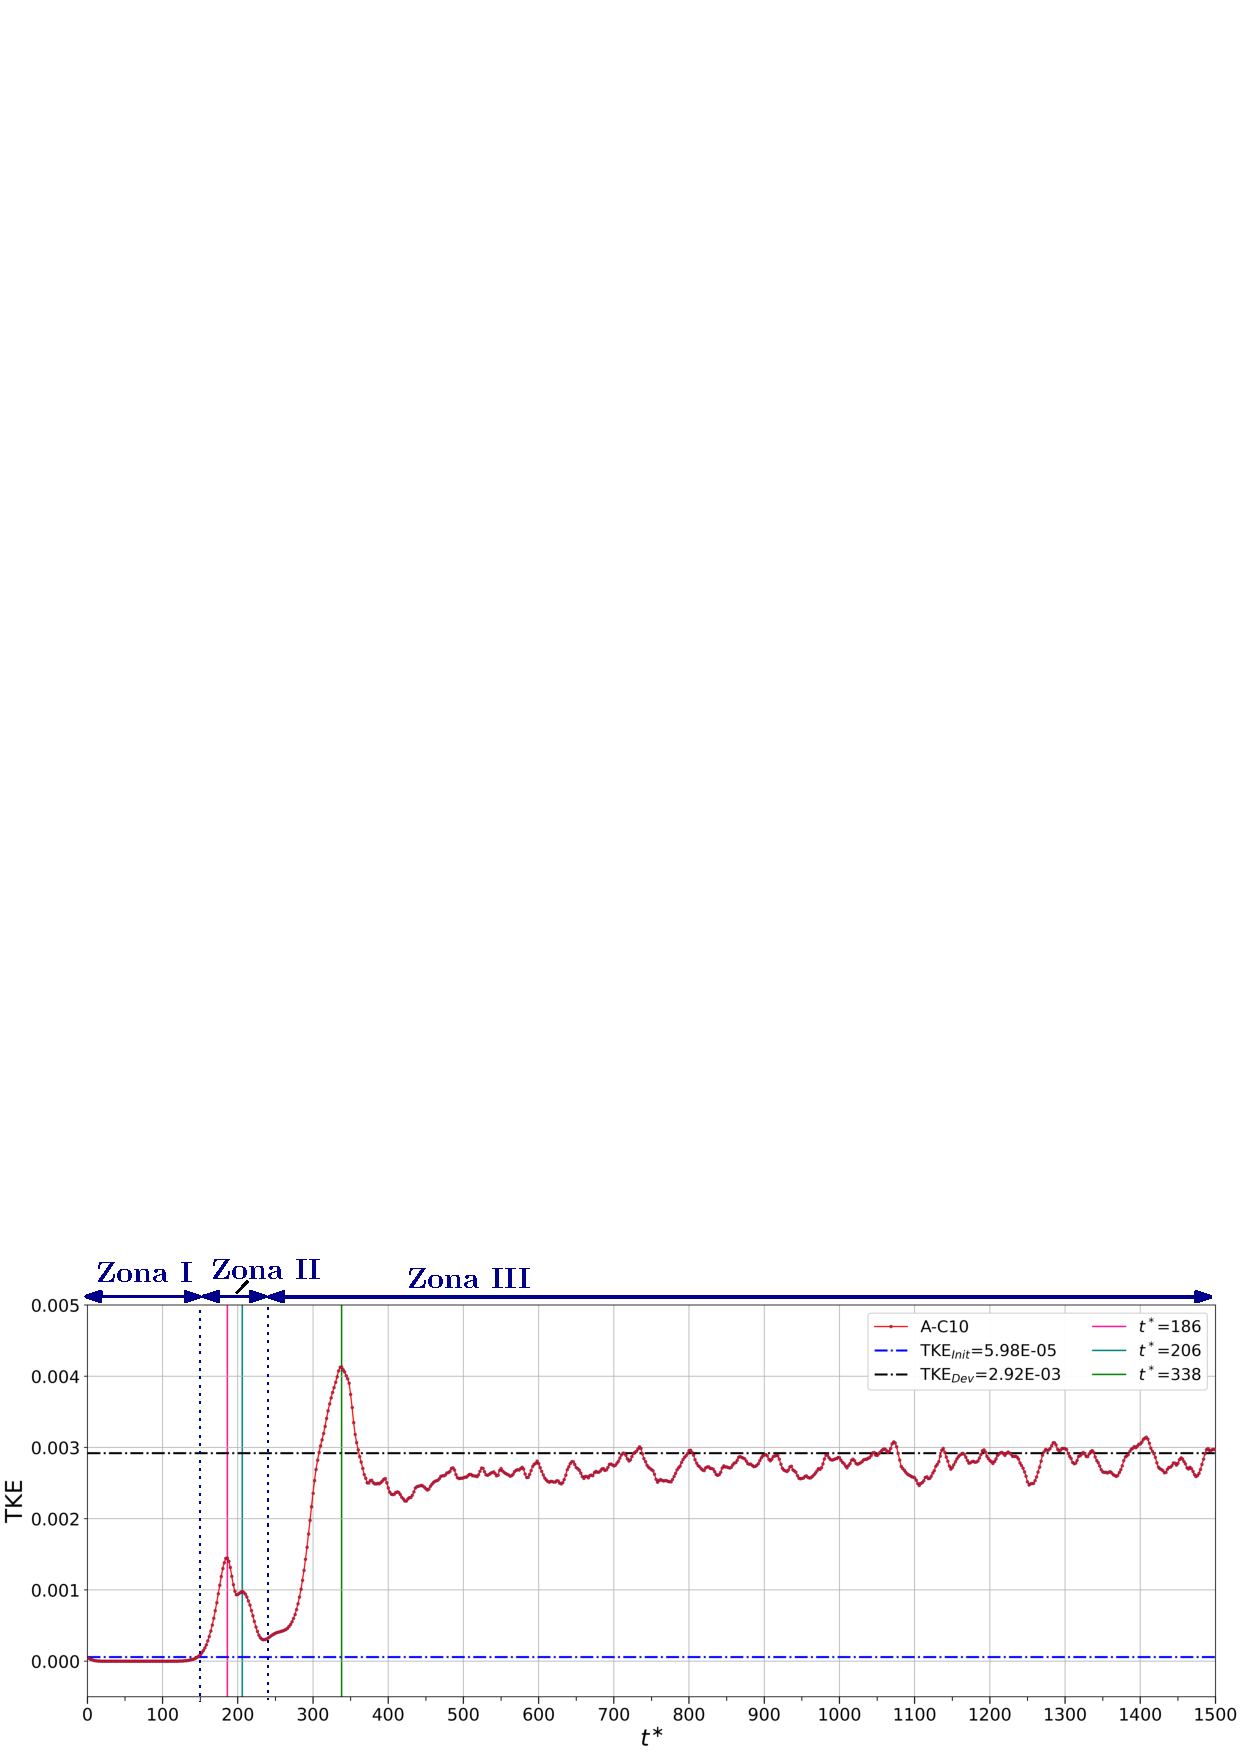
\includegraphics[width=0.49\textwidth]{figures/cap6/Re5000-Pr071-Ri1Em6/Cases_Comp_tke.png}
    \label{fig:tke-Re5000-Pr071}}  
  \subfloat[]{
    \includegraphics[width=0.49\textwidth]{figures/cap6/Re5000-Pr071-Ri1Em6/Cases_Comp_retau.png}
    \label{fig:retau-Re5000-Pr071}}
  \caption{Evolución temporal de \textbf{(a)} TKE y \textbf{(b)} Re$_{\tau}$ para las distintas condiciones iniciales del caso A.}
  \label{fig:case-A-Re5000-Pr071}
\end{figure}



\subsection{Caso B (Ri$_b$=1.06)}

Los parámetros de las perturbaciones utilizadas para la construcción de las condiciones iniciales se resumen en la Tabla \ref{tab:grupo2}. Los ensayos B‑C2 y B‑C3 utilizan únicamente una onda bidimensional ($\text{A}_{\text{2D}}=2 \%$) con diferente autovalor y autofunción, mientras que B‑C4 y B‑C5 añaden una combinación de ondas oblicuas 3D de pequeña amplitud ($\text{A}_{\text{3D}}= 0\text{.}4\%$). En la Figura \ref{fig:case-B-Re5000-Pr071} se expone la evolución en el tiempo de TKE y Re$_{\tau}$ para las distintas condiciones iniciales consideradas.  

En los cuatro ensayos, todas las perturbaciones mencionadas inducen la transición del flujo. Tanto la energía cinética turbulenta como el Re$_{\tau}$ experimentan un crecimiento abrupto en una etapa muy temprana de la transición ($t^*\lesssim 30$). En el caso de Re$_{\tau}$, los máximos se alcanzan para $t^*\lesssim 60$. En particular, en el ensayo B‑C4, el pico se produce casi en la mitad del tiempo ($t^*\approx 25$) que en el resto de los ensayos. Esta cuestión coincide con el hecho de que la parte imaginaria de su autovalor 2D es positiva en comparación al resto de casos que resulta negativa; es decir, se tiene un modo que es más inestable. Luego, para $t^* \gtrsim 150$, el Re$_{\tau}$ se estabiliza en torno a un valor próximo a 270, lo que indica que se ha alcanzado un nuevo estado de flujo. De acuerdo a la línea a trazos (negra) graficada, correspondiente al flujo turbulento del caso completamente desarrollado, se puede afirmar que el flujo transicionó hacia un régimen turbulento.  

Por su parte, la evolución de la TKE comparte ciertos rasgos a los descritos para Re$_{\tau}$. En el ensayo B-C4, el pico se alcanza casi en la mitad del tiempo que en el resto de casos ($t^*\approx 50$); para $t^* \gtrsim 100$, la energía cinética turbulenta se reduce y permanece en torno a un valor constante, $\kappa \approx 0\text{.}002$, que corresponde al caso completamente desarrollado, corroborando también que efectivamente el sistema ha alcanzado un estado de flujo turbulento. Un detalle a destacar es que, mientras en la TKE el máximo alcanzado en el ensayo B-C4 supera al de los demás casos, en el Re$_{\tau}$ ocurre lo contrario: el pico correspondiente al caso B-C4 resulta menor que los picos de los demás ensayos. Se presume que el aumento de la tensión de corte en B-C4 no resulta tan efectivo como en los casos B-C2, B-C3 y B-C5 debido a la gran producción de turbulencia que actúa difundiendo el momento. Por último, para los tiempos adimensionales tales que $t^* > 100$, todas las curvas colapsan, indicando que la dinámica final del sistema, en el estado estadísticamente estacionario, no depende de la perturbación inicial impuesta. 


\paragraph{Caso representativo.} En todos los ensayos del Caso B se logra que el sistema transicione al régimen turbulento. En cada uno se observa un crecimiento, un pico y un decaimiento que tiende al estado turbulento. Se elige el ensayo B‑C2 ya que su transición se alcanza con una perturbación bidimensional  únicamente, a diferencia de lo ocurrido con el caso A.   

\begin{table}[H]
\centering
\caption{Parámetros de las condiciones iniciales para el caso B (Re$_o$ = 5000, Pr = 0.71, Ri$_b$ = 1.06).}
\label{tab:grupo2}
\resizebox{0.75\textwidth}{!}{%
\begin{tabular}{lcccccc}
\toprule
Nomenclatura & $\alpha$ &   $\beta$ &   A$_{2D}$ [\%] &  A$_{3D}$ [\%] & $c_{2D}$ & $c_{3D}$ \\
\midrule
B‑C2 & 1.12 & 0   & 2 & 0   & 0.800 - 0.495 j & - \\
B‑C3 & 1.12 & 0   & 2 & 0   & 2.853 - 0.107 j & - \\
B‑C4 & 1.12 & 2.1 & 2 & 0.4 & 2.315 + 0.424 j & 1.721 + 0.235 j \\
B‑C5 & 1.12 & 2.1 & 2 & 0.4 & 2.853 - 0.107 j & 1.550 + 0.023 j \\
\bottomrule
\end{tabular}}
\end{table}

\begin{figure}[H]
  \centering  
  \subfloat[]{
    \includegraphics[width=0.49\textwidth]{figures/cap6/Re5000-Pr071-Ri1Em4/Cases_Comp_retau.png}
    \label{fig:retau-Re5000-Pr071}}
  \subfloat[]{
    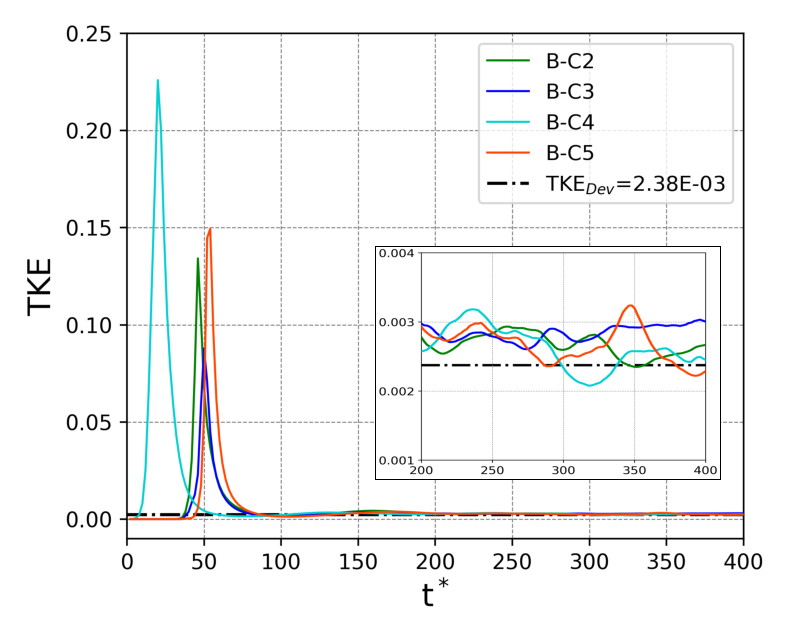
\includegraphics[width=0.49\textwidth]{figures/cap6/Re5000-Pr071-Ri1Em4/Cases_Comp_tke.eps}
    \label{fig:tke-Re5000-Pr071}}

  \caption{Evolución temporal de \textbf{(a)} Re$_{\tau}$ y \textbf{(b)} TKE para las distintas condiciones iniciales del caso B.}
  \label{fig:case-B-Re5000-Pr071}
\end{figure}

\newpage

\section{Análisis detallado del caso A-C10} \label{sec:ac10}

\subsection{TKE y Varianza de la temperatura adimensional}

En las Figuras \ref{fig:tke-ac10} y \ref{fig:tetavar-ac10} la evolución temporal de las magnitudes consideradas (curva roja) se separa en cuatro zonas diferenciadas. A modo de referencia se añaden los valores constantes asociados a la condición inicial y al flujo turbulento completamente desarrollado.

\begin{itemize}
\item \textbf{Zona I (0 $\lesssim$ $\mathbf{t^*}$ $\lesssim$ 150).} Ambas magnitudes experimentan un leve descenso al inicio, luego permanecen prácticamente constantes, sin incrementos ni descensos, y posteriormente aumentan hasta recuperar sus valores iniciales. En este tramo, ambas magnitudes permanecen por debajo de los valores completamente desarrollados del caso turbulento correspondiente. En este intervalo las perturbaciones iniciales no modifican significativamente el flujo base.

\item \textbf{Zona II (150 $\lesssim$ $\mathbf{t^*}$ $\lesssim$ 234)}. La energía cinética turbulenta presenta dos máximos locales bien definidos en torno a $t^*\approx186$ y $t^*\approx206$, separados por un valle intermedio. Por su parte, la varianza de la temperatura experimenta una evolución similar en el mismo intervalo temporal: crece tres órdenes de magnitud, presenta un máximo local, desciende hasta un valle y crece hasta un segundo máximo de menor intensidad. Luego, ambas magnitudes descienden parcialmente antes de volver a crecer.

\item \textbf{Zona III (234 $\lesssim$ $\mathbf{t^*}$ $\lesssim$ 338).} Tanto la TKE, como $\langle \theta^{* \prime} \theta^{* \prime} \rangle$ crecen de forma sostenida, con un cambio de pendiente que ocurre alrededor de $t^*\approx276$. Luego, la TKE alcanza un máximo absoluto en torno a $t^*\approx338$ ($\kappa_{max} \approx 4\text{.}1 \times 10^{-3}$) y la varianza alcanza su máximo absoluto cerca de $t^*\approx320$ con un valor alrededor de $\langle \theta^{* \prime} \theta^{* \prime} \rangle_{\text{max}} \approx 2 \times 10^{4}$. En este intervalo se observa la influencia de la perturbación 3D, que produce un nuevo crecimiento descripto conceptualmente por la inestabilidad secundaria.

\item \textbf{Zona IV ($\mathbf{t^*} \gtrsim 338$).} En una primera etapa, la energía cinética turbulenta desciende desde su valor máximo hasta quedar por debajo del valor constante del caso turbulento completamente desarrollado; posteriormente, aumenta y fluctúa en torno a dicho valor, dentro del rango $\left[ 2\text{.}5 \text{ , } 3\text{.}5 \right] \times 10^{-3}$. Por su parte, la varianza de la temperatura desciende de manera gradual, acercándose al valor de referencia del caso turbulento desarrollado.
\end{itemize}

\newpage

\begin{figure}[H]
  \centering  
  \subfloat[]{
    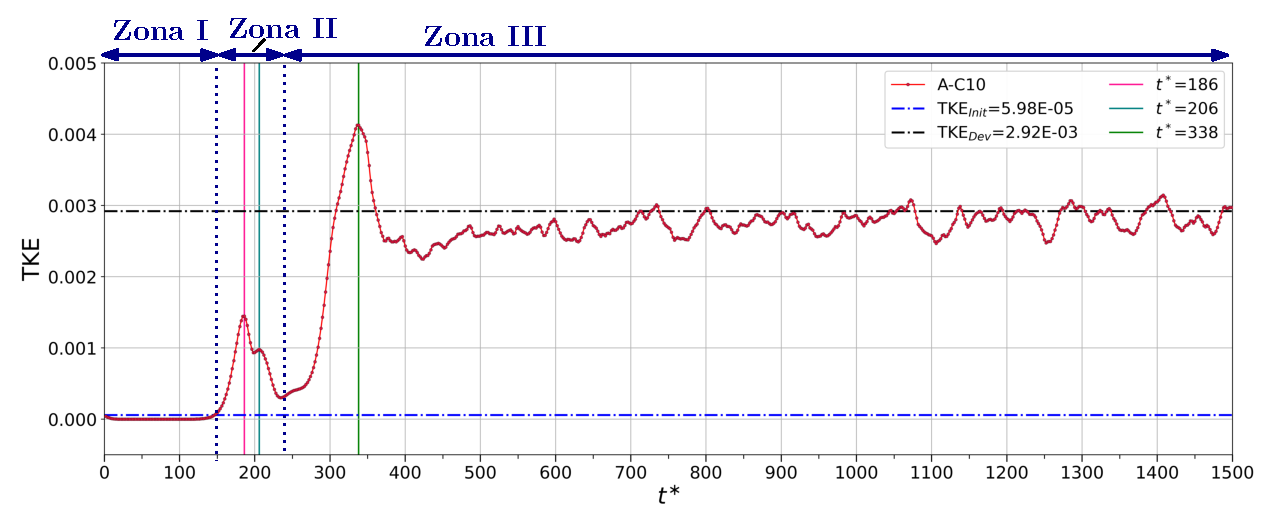
\includegraphics[width=0.9\textwidth]{figures/cap6/A-C10/Cases_Comp_tke.eps}
    \label{fig:tke-ac10}}
    
  \subfloat[]{
    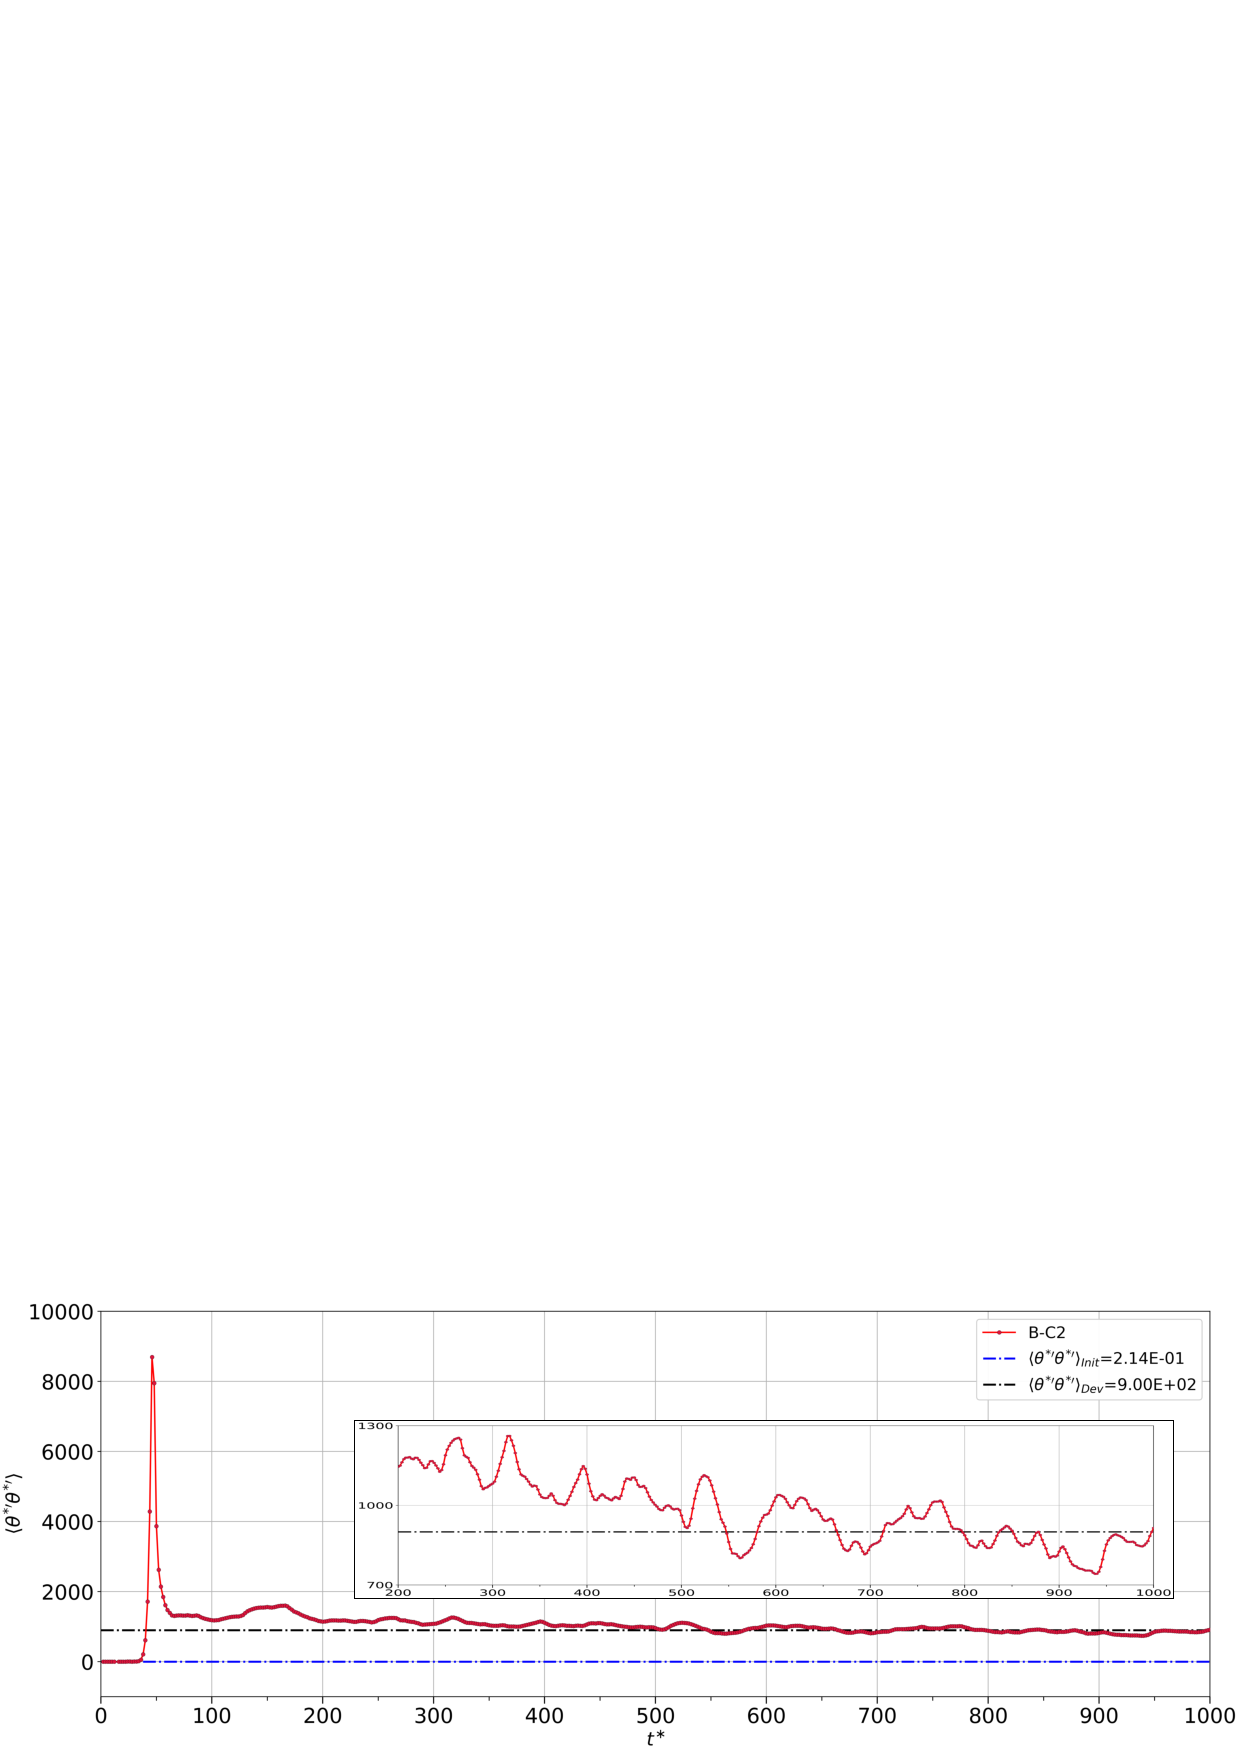
\includegraphics[width=0.9\textwidth]{figures/cap6/A-C10/Cases_Comp_tetavar.png}
    \label{fig:tetavar-ac10}}
  \caption{Evolución temporal de \textbf{(a)} la energía cinética turbulenta y \textbf{(b)} la varianza de la temperatura, para el caso A-C10.}
  \label{fig:ac10-2}
\end{figure}

\subsection{Perfiles de velocidad y temperatura}

En las Figuras \ref{fig:uxs-ac10} y \ref{fig:phis-ac10} se muestran, respectivamente, los perfiles de velocidad y \linebreak temperatura adimensional para $t^*=2$, $186$, $206$, $338$, $750$, $1500$ (de izquierda a derecha). A modo de referencia, se incluye el perfil correspondiente al flujo turbulento completamente \linebreak desarrollado. Los instantes elegidos abarcan la etapa laminar inicial ($t^*=2$), los máximos locales ($t^* \approx 186$ y $t^* \approx 206$), el máximo absoluto de la TKE y dos tiempos en los que el flujo ya es turbulento.

La perturbación impuesta modifica el perfil de velocidad que en un inicio tiene forma de ``M'' (véase Sección \ref{sec:mix-laminar}). A medida que el flujo evoluciona se observa que en $t^* \approx 186$ y $t^* \approx 206$, los perfiles conservan la simetría pero no mantienen su forma característica inicial. Esta forma relativamente más plana en los perfiles es consecuencia de un aumento de la difusión de momento dada por el incremento de turbulencia (véase Figura \ref{fig:tke-ac10}). Asimismo, próximo a $t^* \approx 338$, se aprecia una aparente ``pérdida'' en la simetría del perfil. En una etapa ya turbulenta, los perfiles de velocidad se aproximan a aquel correspondiente al flujo completamente desarrollado. Los perfiles de temperatura adimensional siguen una evolución análoga: se deforman manteniendo su simetría, luego la misma se desvanece momentáneamente en $t^* \approx 338$ (el perfil se vuelve asimétrico), y posteriormente tienden hacia el perfil del caso turbulento desarrollado. El efecto de la turbulencia aplana los perfiles de temperatura y aproxima la temperatura en el centro del canal al valor de aquella impuesta en la pared. Por otro lado, al inspeccionar los perfiles de velocidad y temperatura en conjunto, se observa que el desarrollo de la parte hidrodinámica se encuentra ligeramente acelerado respecto al desarrollo térmico. Este hecho depende del número de Prandtl (Pr) y de cuán relevante es la boyancia en la ecuación de momento (Ri$_b$).


\begin{figure}[H]
  \centering  
  \subfloat[]{
    \includegraphics[width=1.05\textwidth]{figures/cap6/A-C10/ux_profiles_mosaic.png}
    \label{fig:uxs-ac10}}
  
  \subfloat[]{
    \includegraphics[width=1.05\textwidth]{figures/cap6/A-C10/phi_profiles_mosaic.png}
    \label{fig:phis-ac10}}
  \caption{Perfiles de \textbf{(a)} velocidad y \textbf{(b)} temperatura adimensional para distintos instantes $t^*$ correspondientes al caso A-C10.}
  \label{fig:mosaico-ac10}
\end{figure} 

Respecto a la pérdida momentánea de simetría mostrada en los perfiles de la Figura \ref{fig:mosaico-ac10}  se especula que se debe a un efecto de dominio. Un dominio que abarque más de una longitud de onda de las perturbaciones iniciales, en las direcciones $X$ y $Z$, podría compensar este efecto. %Por cuestiones de costo computacional la verificación de esta hipótesis queda para estudios futuros.

Con el fin de profundizar en el entendimiento de la aparente pérdida de simetría observada en los perfiles para el instante $t^* = 338$, resulta ilustrativo examinar las estructuras de vórtices del flujo. Dichas estructuras se obtienen mediante el ``Criterio Q'' \cite{hunt1988eddies}. El análisis que se realiza a continuación se hace con un enfoque cualitativo. En la Figura \ref{fig:mosaico2-ac10} se exponen capturas de las ``isosuperficies de Q'' para tres tiempos distintos: $t^* = 186$ (Figuras \ref{fig:t186-xy-ac10} y  \ref{fig:t186-zy-ac10}),  $t^* = 338$  (Figuras \ref{fig:t338-xy-ac10} y  \ref{fig:t338-zy-ac10}) y  $t^* = 1500$  (Figuras \ref{fig:t1500-xy-ac10} y  \ref{fig:t1500-zy-ac10}); las capturas ubicadas a la derecha corresponden a la vista del dominio desde un punto de vista normal a los planos $ZY$, mientras que las ubicadas a la izquierda muestran la vista normal a los planos $XY$.

En el instante $t^* = 186$, se observa una estructura coherente y ordenada, asociada a las ondas TS; esto es consistente con el hecho de que los perfiles en la condición inicial tengan una simetría respecto a la dirección $Y$ (antes de que ocurra el máximo absoluto de la TKE). 

\newpage

En el segundo instante considerado (Figuras \ref{fig:t338-xy-ac10} y \ref{fig:t338-zy-ac10}), las capturas revelan una mayor presencia de estructuras de vórtices en la pared superior ($\text{y}=2$) respecto a la inferior ($\text{y}=0$); esto último se puede corroborar mirando capturas adicionales en las Figuras \ref{fig:t338-v1-ac10} y \ref{fig:t338-v2-ac10} que muestran el dominio desde otros puntos de vista. Este ``desbalance'' de estructuras da sustento a la idea supuesta de ``pérdida en la simetría'' de los perfiles de velocidad y temperatura antes mencionada. Nótese (Figura \ref{fig:t338-zy-ac10}), que si bien las estructuras ya no son simétricas respecto al plano $ZX$\footnote{En esta captura, la posición de este plano se encuentra en Y=1.} en $y^*=0$ (representado por la línea azul) se puede apreciar cierta simetría respecto al plano $XY$\footnote{En esta captura, la posición de este plano se encuentra en Z=1.5.} en $z^*= 1 \text{.} 5$ (señalado por la línea roja). En este sentido, todavía se puede considerar que, en $t^* = 338$, el flujo conserva cierto grado de orden y coherencia. 


En el último instante, donde el flujo ya se ha desarrollado y se encuentra en estado estadísticamente estacionario, las estructuras han dejado de ser coherentes y tienden a organizarse cerca de las paredes, en consistencia con los perfiles simétricos característicos de los flujos turbulentos completamente desarrollados \cite{machaca2024}.

\begin{figure}%[H]
  \centering  
  \subfloat[]{
    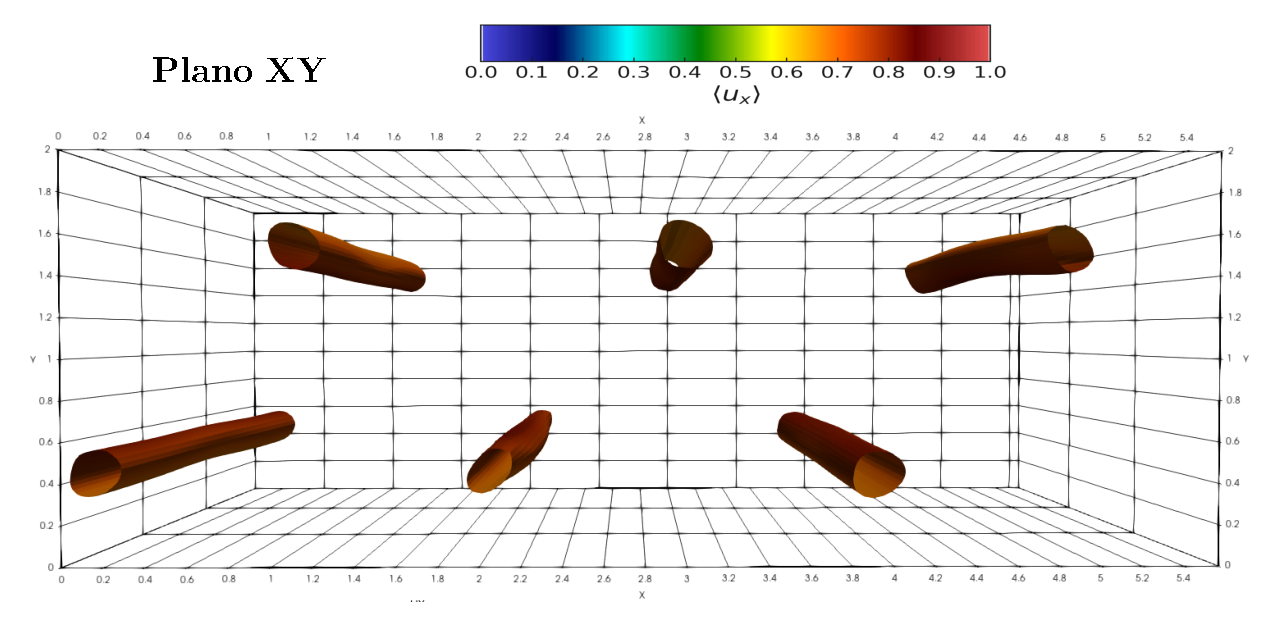
\includegraphics[width=0.58\textwidth]{figures/cap6/A-C10/screenshots_times/t186_xy.eps}
    \label{fig:t186-xy-ac10}}  
  \subfloat[]{
    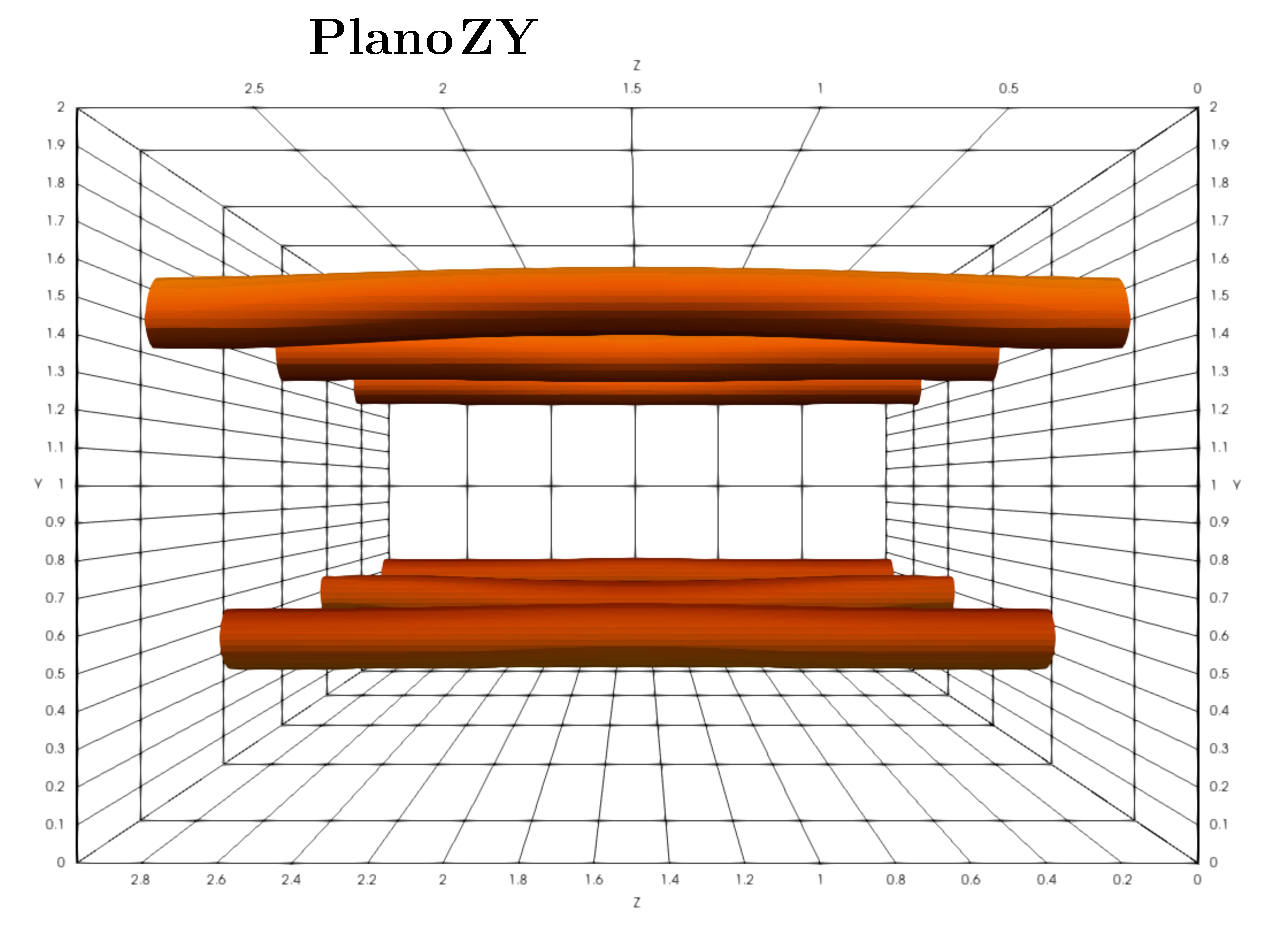
\includegraphics[width=0.40\textwidth]{figures/cap6/A-C10/screenshots_times/t186_zy.eps}
    \label{fig:t186-zy-ac10}}
    
  \subfloat[]{  
    \includegraphics[width=0.58\textwidth]{figures/cap6/A-C10/screenshots_times/t338_xy.png}
    \label{fig:t338-xy-ac10}}  
  \subfloat[]{
    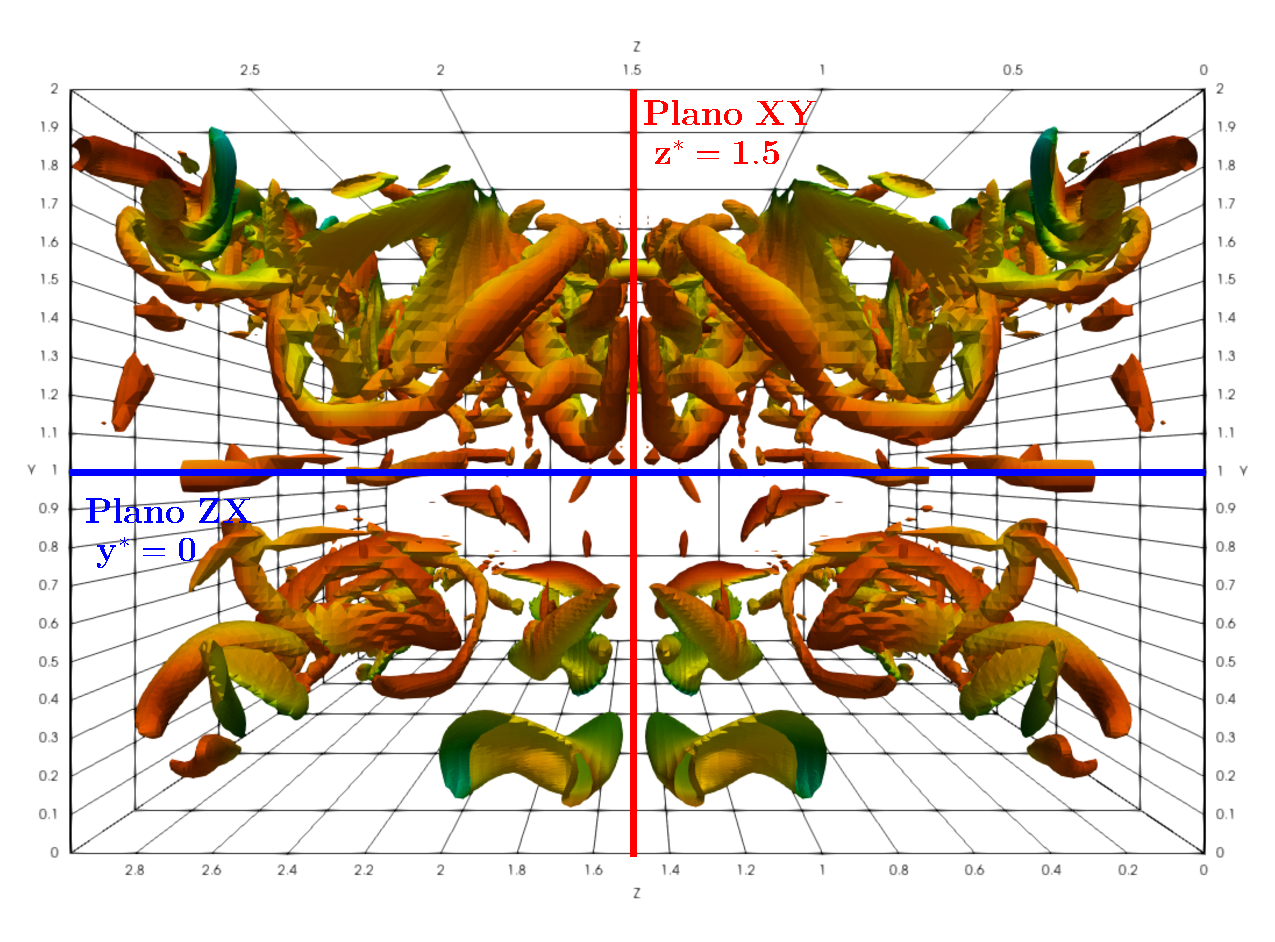
\includegraphics[width=0.40\textwidth]{figures/cap6/A-C10/screenshots_times/t338_zy.eps}
    \label{fig:t338-zy-ac10}}
  
  \subfloat[]{ 
    \includegraphics[width=0.58\textwidth]{figures/cap6/A-C10/screenshots_times/t1500_xy.png}
    \label{fig:t1500-xy-ac10}}  
  \subfloat[]{
    \includegraphics[width=0.40\textwidth]{figures/cap6/A-C10/screenshots_times/t1500_zy.png}
    \label{fig:t1500-zy-ac10}}
  \caption{Ensayo A-C10. Capturas de las estructuras de vórtices para tres instantes de tiempo: $t^* =186$ con $Q=0\text{.}1$ (\textbf{(a)} y \textbf{(b)}), $t^* =338$ con $Q=0\text{.}5$ (\textbf{(c)} y \textbf{(d)}) y $t^* = 1500$ con $Q=0\text{.}5$ (\textbf{(e)} y \textbf{(f)}). Aquí $Q$ hace referencia al parámetro del Criterio Q. \textit{Observación: la escala de colores de la captura en \textbf{(a)} se aplica al resto de figuras}.}
  \label{fig:mosaico2-ac10}
\end{figure}

\begin{figure}%[H]
  \centering  
  \subfloat[]{
    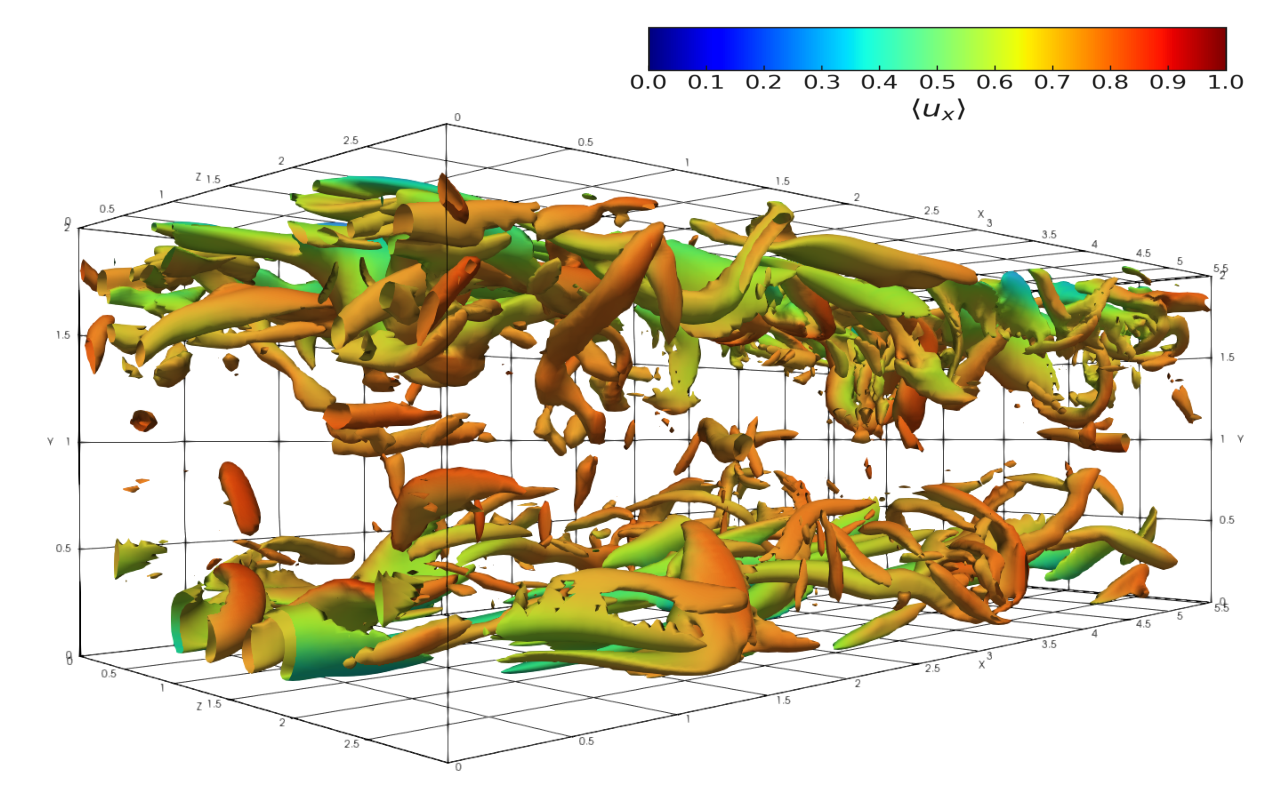
\includegraphics[width=0.49\textwidth]{figures/cap6/A-C10/screenshots_times/t338_v1.eps}
    \label{fig:t338-v1-ac10}}
  \subfloat[]{
    \includegraphics[width=0.49\textwidth]{figures/cap6/A-C10/screenshots_times/t338_v2.png}
    \label{fig:t338-v2-ac10}}
  \caption{Capturas adicionales de las estructuras de vórtices para $t^* =338$ desde otros puntos de vista ($Q=0\text{.}5$).}
  \label{fig:mosaico-ac10-v1-v2}
\end{figure}

\subsection{Factor de fricción de Darcy y número de Nusselt}
En la Figura \ref{fig:darcy-ac10} se presenta la evolución temporal del factor de fricción de Darcy. En la \textbf{Zona I} ($0 < t^* < 150$), $f$ permanece prácticamente constante y coincide con el \linebreak valor inicial/laminar\footnote{Recuérdese que los valores de $f$ y Nu obtenidos a partir de la solución laminar y de la condición inicial resultan equivalentes.} (línea a trazos azul). En las \textbf{Zonas II} y \textbf{III}, y parte de la \textbf{Zona IV} ($150 \lesssim t^* \lesssim 352 $), se observa primero una disminución suave hasta un mínimo de $f=0\text{.}0167$ en $t^*\approx270$, seguida de un incremento pronunciado que alcanza su máximo en $t^*\approx352$ ($f \approx 0\text{.}037$). A partir de ese pico, y en el resto de la \textbf{Zona IV} ( $t^*\gtrsim352$), $f$ desciende y se estabiliza entre los valores 0.0275 y 0.033, en torno al valor de referencia del caso completamente desarrollado (línea a trazos negra). De esta forma, es posible distinguir con claridad la etapa transitoria y el posterior establecimiento de un régimen turbulento que persiste en el tiempo.

Por último, la Figura \ref{fig:nu-ac10} presenta la evolución temporal del número de Nusselt. El valor se mantiene prácticamente constante y coincidente con la solución laminar hasta $t^* \approx 300$. A partir de allí, crece de manera monótona hasta el final de la simulación. La magnitud tiende al valor correspondiente al régimen turbulento desarrollado (convección mixta); sin embargo, el tiempo físico simulado no resulta suficiente para garantizar la convergencia. Esta misma situación puede observarse en la varianza de la temperatura y en el perfil de temperatura para $t^*=1500$ aunque no de manera tan marcada como en el caso de Nu. Esto sugiere que se requiere extender la simulación para que las magnitudes térmicas alcancen su estado estadísticamente estacionario.

\begin{figure}[H]
  \centering  
  \subfloat[]{
    \includegraphics[width=0.9\textwidth]{figures/cap6/A-C10/Cases_Comp_darcy.png}
    \label{fig:darcy-ac10}}
    
  \subfloat[]{
    \includegraphics[width=0.9\textwidth]{figures/cap6/A-C10/Cases_Comp_nussel.png}
    \label{fig:nu-ac10}}
  \caption{Evolución temporal de \textbf{(a)} factor de fricción de Darcy y \textbf{(b)} número de Nusselt, para el caso A-C10.}
  \label{fig:ac10-1}
\end{figure}



\newpage
\section{Análisis detallado del caso B‑C2} \label{sec:bc2}

\subsection{TKE y varianza de la temperatura adimensional}
En las Figuras \ref{fig:tke-bc2} y \ref{fig:tetavar-bc2} se expone, respectivamente, la evolución temporal de la energía cinética turbulenta (TKE) y la varianza de la temperatura; dicha evolución se separa en tres regiones. Se añaden valores constantes de referencia asociados al cálculo de dichas cantidades empleando la condición inicial y el flujo turbulento en estado estadísticamente estacionario.

\begin{itemize}

  \item \textbf{Zona I ($0 \lesssim \mathbf{t^*} \lesssim 32$).} Ambas cantidades se mantienen prácticamente constantes y coinciden con su valor de referencia asociado a la condición inicial. El sistema no transiciona.

  \item \textbf{Zona II ($32 \lesssim \mathbf{t^*} \lesssim 100$).} Aquí, la TKE crece y alcanza un máximo absoluto en $t^* \approx 46$ ($\kappa_{\text{max}}$ $\approx 0\text{.}134$). De forma similar, la varianza de la temperatura crece hasta que alcanza un máximo absoluto en el mismo instante de tiempo que la TKE, con un valor $\langle \theta^{*\prime} \theta^{*\prime}\rangle_{\text{max}} \approx 8700$. A partir de $t^* \approx 46$, ambas magnitudes decrecen sin retornar a los valores iniciales, y tienden hacia el estado estadísticamente estacionario del flujo turbulento correspondiente.

% NO BORRAR
%  \item \textbf{Zona II ($32 \lesssim \mathbf{t^*} \lesssim 100$).} Aquí, la TKE crece y alcanza un máximo absoluto en $t^* \approx 46$ ($k_{\text{max}}$ $\approx 0\text{.}134$), superando en dos órdenes de magnitud al valor registrado en el ensayo A-C10. De forma similar, la varianza de la temperatura crece hasta que alcanza un máximo absoluto en el mismo instante de tiempo que la TKE, con un valor $\langle \theta^{*\prime} \theta^{*\prime}\rangle_{\text{max}} \approx 8700$, siendo casi un orden de magnitud menor que en el ensayo A-C10. A partir de $t^* \approx 46$, ambas magnitudes decrecen sin retornar a los valores iniciales, y tienden hacia el estado estadísticamente estacionario del flujo turbulento correspondiente.

  \item \textbf{Zona III ($\mathbf{t^*} \gtrsim 100$).} En esta etapa, ambas magnitudes experimentan un segundo máximo local, de mucha menor intensidad, en $t^* \approx 160$. Luego, para $t^* > 200$, ambas cantidades fluctúan en torno a las magnitudes constantes de referencia: la TKE se mantiene acotada entre 0.002 y 0.003, mientras que la varianza de la temperatura se encuentra entre 700 y 1300. Para $t^* >200$, el sistema tiende hacia un nuevo estado de flujo, es decir, uno turbulento. 

\end{itemize}


\begin{figure}[H]
  \centering  
    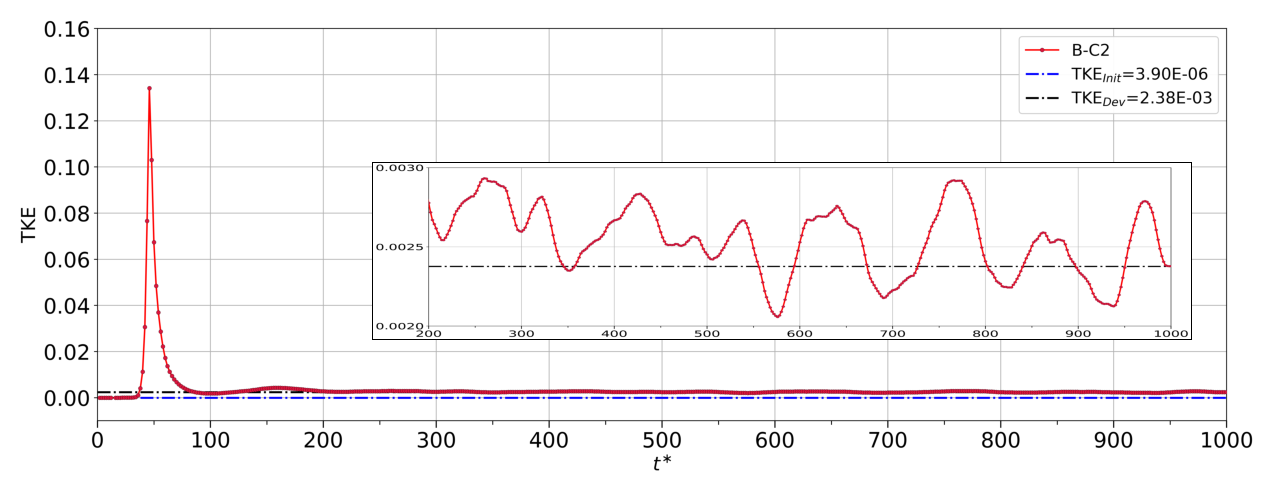
\includegraphics[width=0.9\textwidth]{figures/cap6/B-C2/Cases_Comp_tke.eps}
   \caption{Evolución temporal de la energía cinética turbulenta para el caso B-C2.}
    \label{fig:tke-bc2}
\end{figure}

\newpage

\begin{figure}[H]
  \centering      
    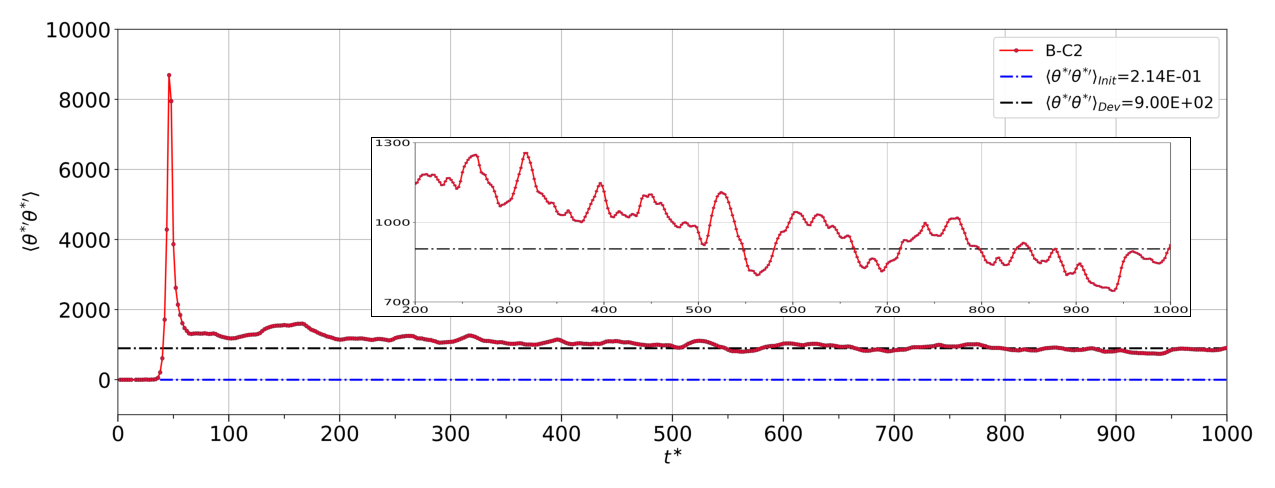
\includegraphics[width=0.9\textwidth]{figures/cap6/B-C2/Cases_Comp_tetavar.eps}
     \caption{Evolución temporal de la varianza de la temperatura para el caso B-C2.}
      \label{fig:tetavar-bc2}
\end{figure}

\subsection{Perfiles de velocidad y temperatura}
En las Figuras \ref{fig:uxs-bc2} y \ref{fig:phis-bc2} se presentan, respectivamente, los perfiles de velocidad y de temperatura adimensional para $t^*$ = 2, 46, 160, 500, 1000 (de izquierda a derecha). Como referencia, se incluye el perfil correspondiente al flujo completamente desarrollado en convección mixta. La selección de tiempos abarca el régimen laminar inicial ($t^* = 2$), el máximo absoluto en $t^* \simeq 46$, el máximo local subsiguiente de mucha menor intensidad, en $t^* \simeq 160$, y dos instantes posteriores en los que el flujo ya se encuentra en régimen turbulento.

En la etapa inicial, el perfil exhibe la simetría característica de la solución laminar en forma de ``M''. En torno al máximo absoluto de la TKE, los perfiles se ensanchan levemente y muestran, nuevamente, una aparente pérdida de simetría. A medida que aumenta el tiempo adimensional, los perfiles de ambas magnitudes convergen hacia las soluciones de referencia del flujo completamente desarrollado. Al compararse con el ensayo A-C10 (Figura \ref{fig:phis-ac10}), se observa que el aumento de la fuerza boyante tiene por efecto acelerar la evolución del campo de temperaturas, favoreciendo una convergencia más rápida hacia el flujo completamente desarrollado.


Nuevamente, se analizan las estructuras de vórtices mediante un enfoque cualitativo, con la intención de entender la aparente pérdida de simetría en los perfiles que ocurre a $t^* = 46$. En la Figura \ref{fig:mosaico2-bc2} se exponen capturas de las isosuperficies de Q asociadas a tres tiempos distintos: $t^* = 2$ (Figuras \ref{fig:t2-xy-bc2} y  \ref{fig:t2-zy-bc2}),  $t^* = 46$  (Figuras \ref{fig:t46-xy-bc2} y \ref{fig:t46-zy-bc2}) y  $t^* = 500$  (Figuras \ref{fig:t500-xy-bc2} y \ref{fig:t500-zy-bc2}). Obsérvese que las capturas ubicadas a la derecha corresponden a la vista del dominio desde un punto de vista normal a los planos $ZY$, mientras que las ubicadas a la izquierda muestran la vista normal a los planos $XY$.

\newpage

\begin{figure}[H]
  \centering  
  \subfloat[]{
    \includegraphics[width=1.02\textwidth]{figures/cap6/B-C2/ux_profiles_mosaic.png}
    \label{fig:uxs-bc2}}
  
  \subfloat[]{
    \includegraphics[width=1.02\textwidth]{figures/cap6/B-C2/phi_profiles_mosaic.png}
    \label{fig:phis-bc2}}
  \caption{Perfiles de \textbf{(a)} velocidad y \textbf{(b)} temperatura adimensional para distintos instantes $t^*$ correspondiente al caso B-C2.}
    \label{fig:mosaico-bc2}
\end{figure}




En el instante $t^* = 2$, se observa una estructura coherente y ordenada, asociada a las ondas TS. Esto es consistente con la simetría de los que perfiles en la condición inicial; asimismo, dichas estructuras se posicionan muy cerca de las paredes al igual que ocurre con los máximos del perfil de velocidad.

En el segundo instante de tiempo considerado, se observa que las estructuras no se \linebreak aglomeran de forma simétrica respecto a las paredes ($y^*=\pm 1$). Una visualización más clara, se aprecia en las Figuras \ref{fig:t46-zy_x1}-\ref{fig:t46-zy_x5} donde se muestran cortes de planos $ZY$ para $x^*=1,2,4,5$, respectivamente. A partir de estos cortes se observa que, a lo largo de la dirección $X$, las estructuras se distribuyen de manera no uniforme cerca de las paredes. Este ``desequilibrio'' de pequeñas estructuras produce una mezcla no homogénea de las cantidades, lo que podría dar cierto entendimiento, al menos conceptual, del hecho que los máximo del perfil de velocidad cerca las paredes sea levemente distinto en el dominio simulado.   

Por su parte, en el último instante de tiempo considerado (estado estadísticamente estacionario), se aprecia que las estructuras  tienden a aglomerarse cerca de las paredes y también carecen de coherencia y orden (véase Figuras \ref{fig:t500-xy-bc2} y \ref{fig:t500-zy-bc2}). Entonces, dado que la dinámica en ambas paredes es la misma en términos estadísticos, las cantidades de interés resultan, en promedio, simétricas respecto a la dirección $Y$. Esto es consistente con lo observado en el perfil de velocidad \textit{streamwise} (Figura \ref{fig:uxs-bc2} a $t^*=500$).

Resulta evidente que el efecto de la fuerza boyante impacta considerablemente en cómo el fluido evoluciona en el tiempo. Uno de los efectos más notables, como se menciona anteriormente, es la aceleración de la dinámica del sistema. 

\begin{figure} [H]
  \centering  
  \subfloat[]{
    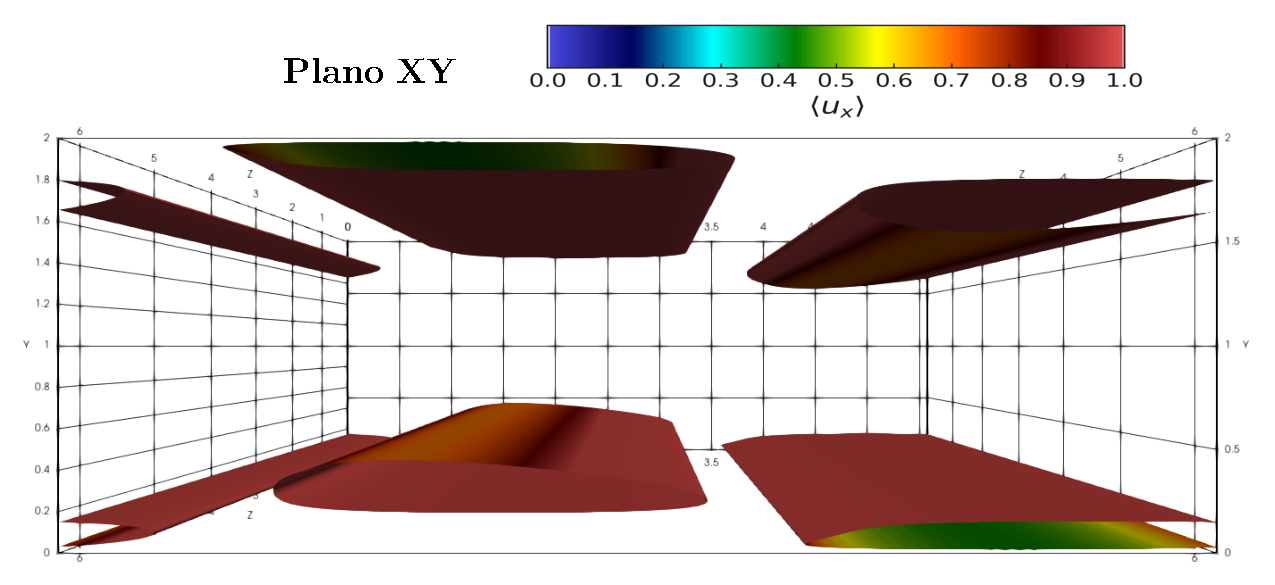
\includegraphics[width=0.48\textwidth]{figures/cap6/B-C2/screenshots_times/t2_xy.eps}
    \label{fig:t2-xy-bc2}}  
  \subfloat[]{
    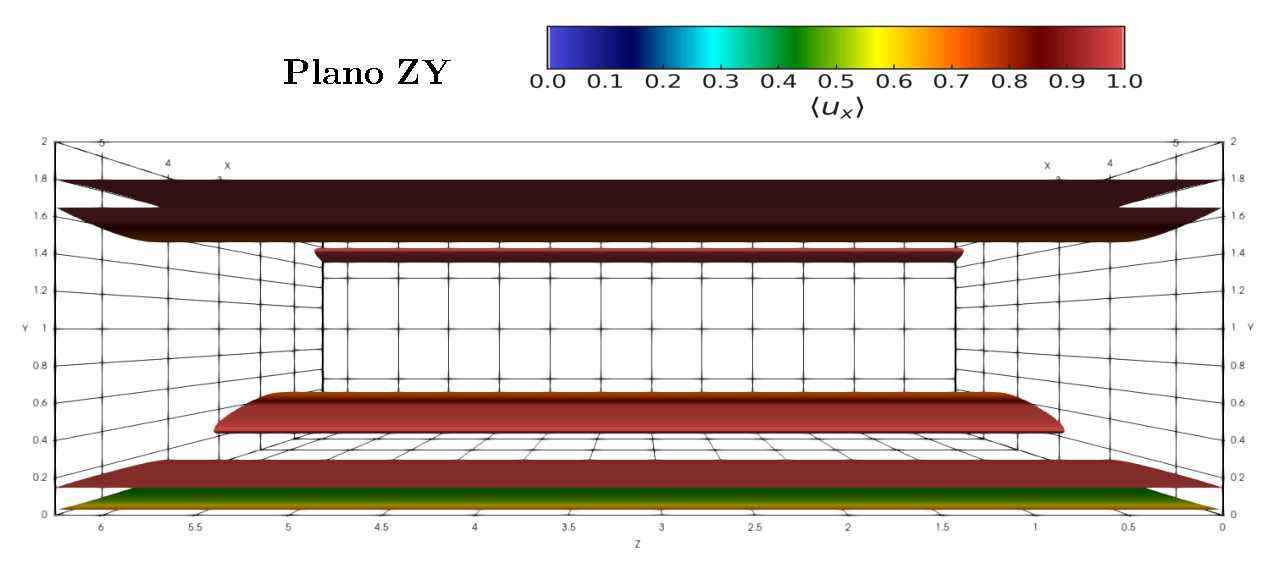
\includegraphics[width=0.5\textwidth]{figures/cap6/B-C2/screenshots_times/t2_zy.eps}
    \label{fig:t2-zy-bc2}}
    
  \subfloat[]{
    \includegraphics[width=0.47\textwidth]{figures/cap6/B-C2/screenshots_times/t46_xy.png}
    \label{fig:t46-xy-bc2}}  
  \subfloat[]{
    \includegraphics[width=0.51\textwidth]{figures/cap6/B-C2/screenshots_times/t46_zy.png}
    \label{fig:t46-zy-bc2}}

  
  \subfloat[]{
    \includegraphics[width=0.47\textwidth]{figures/cap6/B-C2/screenshots_times/t500_xy.png}
    \label{fig:t500-xy-bc2}}  
  \subfloat[]{
    \includegraphics[width=0.51\textwidth]{figures/cap6/B-C2/screenshots_times/t500_zy.png}
    \label{fig:t500-zy-bc2}}
  \caption{Ensayo B-C2. Capturas de las estructuras de vórtices para tres instantes de tiempo: $t^* =2$ con $Q=0\text{.}0005$ (\textbf{(a)} y \textbf{(b)}), $t^* =46$ con $Q=10$ (\textbf{(c)} y \textbf{(d)}) y $t^* = 500$ con $Q=0\text{.}4$ (\textbf{(e)} y \textbf{(f)}). Aquí $Q$ también hace referencia al parámetro del Criterio Q. }
  \label{fig:mosaico2-bc2}
\end{figure}






\subsection{Factor de fricción de Darcy y número de Nusselt}
La Figura \ref{fig:darcy-bc2} muestra la evolución temporal del factor de fricción de Darcy. En las \textbf{Zonas I y II} ($0 \lesssim t^* \lesssim 100$), desde el inicio hasta $t^* \approx 20$, $f$ se mantiene próximo al valor laminar (línea a trazos azul). Entre $t^* \approx 20$ y $t^* \approx 46$ el factor de fricción experimenta dos picos sucesivos antes de culminar en un máximo absoluto de mucho mayor amplitud \linebreak ($f_{\max}$ $\approx$ 0.174). A partir de ese punto, $f$ decrece de manera pronunciada por debajo del valor \linebreak laminar inicial. En la \textbf{Zona III} ($t^* \gtrsim 100$), la curva permanece en torno al valor de la referencia del flujo completamente desarrollado hasta $t^* \approx 400$; luego, la magnitud adquiere valores levemente por debajo del valor de referencia antes mencionado. Esto último es debido a que el sistema necesita más tiempo para desarrollarse. Este efecto se ve más claramente en la siguiente discusión.

La Figura \ref{fig:nu-bc2} muestra la evolución temporal de Nu. Se observa que el número de Nusselt se mantiene cercano a la solución laminar inicial hasta $t^* \approx 34$, luego comienza a decrecer rápidamente hasta un valor mínimo en $t^* \approx 48$ ($\text{Nu}_{\text{min}} \simeq 10\text{.}6$). A partir de allí, Nu comienza un período de crecimiento de manera monótona y sostenida, superando el valor inicial de referencia, tendiendo a la referencia del estado turbulento estadísticamente estacionario. 

\newpage

\begin{figure}[H]
  \centering  
  \subfloat[]{
    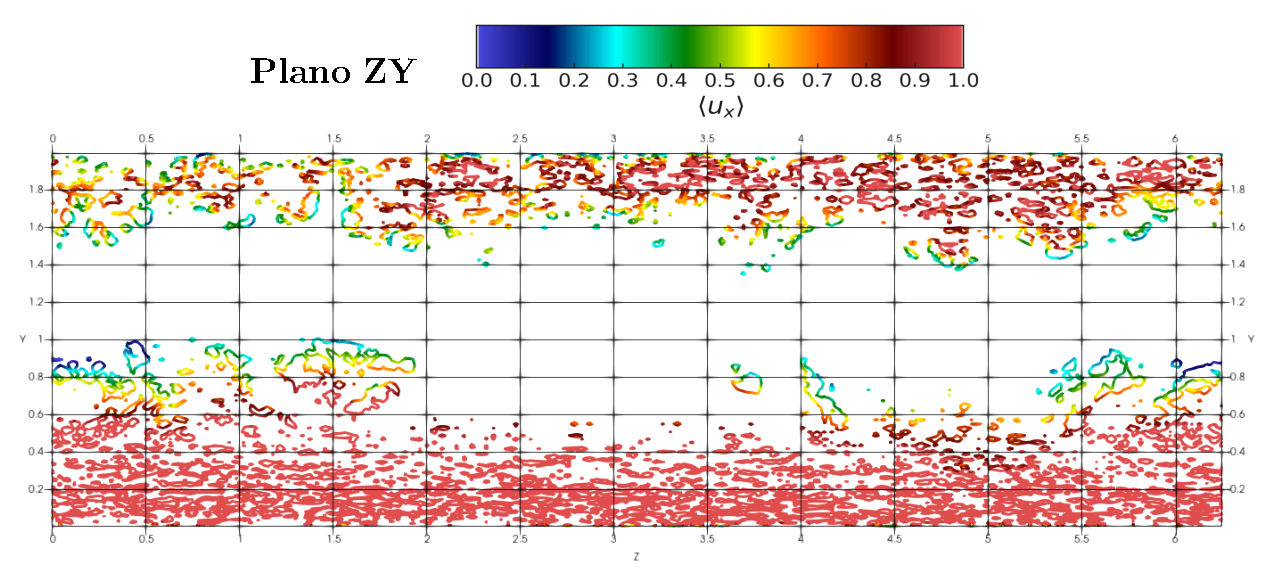
\includegraphics[width=0.49\textwidth]{figures/cap6/B-C2/screenshots_times/zy_x1.eps}
    \label{fig:t46-zy_x1}}  
  \subfloat[]{
    \includegraphics[width=0.49\textwidth]{figures/cap6/B-C2/screenshots_times/zy_x2.png}
    \label{fig:t46-zy_x2}}

  \subfloat[]{
    \includegraphics[width=0.49\textwidth]{figures/cap6/B-C2/screenshots_times/zy_x4.png}
    \label{fig:t46-zy_x4}}  
  \subfloat[]{
    \includegraphics[width=0.49\textwidth]{figures/cap6/B-C2/screenshots_times/zy_x5.png}
    \label{fig:t46-zy_x5}}
    
  \caption{Ensayo B-C2. Cortes de las isosuperficies correspondientes al instante $t^* =46$. Planos $ZY$ para: \textbf{(a)} $x^*=1$, \textbf{(b)} $x^*=2$, \textbf{(c)} $x^*=4$ y \textbf{(d)} $x^*=5$.}
  \label{fig:mosaico3-bc2}
\end{figure}



El valor mínimo que alcanza Nu, coincide aproximadamente con el instante donde TKE es máximo y donde se aprecia, en la Figura \ref{fig:mosaico-bc2}, a $t^*=46$, una gran variación en el perfil de velocidad respecto al correspondiente a $t^*=2$. La TKE ha sido efectiva achatando el perfil de velocidad. Por otro lado, entre estos dos instantes de tiempo, el perfil de temperatura no ha cambiado significativamente, evidenciando un retardo en la evolución del campo de \linebreak temperaturas respecto al observado en la velocidad \textit{streamwise}. Matemáticamente, se aprecia que la temperatura \textit{bulk} (ecuación \ref{eq:tita_bulk}) aumenta entre $t^*=2$ y $t^*=46$ ya que el perfil de velocidad deja de tener peso en los bordes, donde la temperatura es baja, y toma más relevancia en el centro del canal, donde la temperatura es mayor. El incremento en $\langle \theta^*_{b} \rangle$ corresponde a un decrecimiento del Nu. Físicamente, se puede recurrir nuevamente a la analogía de Prandtl \cite{aicher1997}. La difusión de energía por efectos de la turbulencia es, a primer orden, proporcional al gradiente de velocidades entre la capa viscosa y el centro del canal; esta cantidad  disminuye notablemente desde la condición inicial hasta $t^*=46$. Para tiempos mayores, el perfil de temperatura se reduce en forma monótona dando lugar a la reducción de la $\langle \theta^*_{b} \rangle$ o al incremento de Nu.



\begin{figure}[H]
  \centering  
    \includegraphics[width=0.8\textwidth]{figures/cap6/B-C2/Cases_Comp_darcy.png}
   \caption{Evolución temporal del factor de fricción de Darcy para el caso B-C2.}  
    \label{fig:darcy-bc2}
\end{figure}

\newpage

\begin{figure}[H]
  \centering  
    \includegraphics[width=0.8\textwidth]{figures/cap6/B-C2/Cases_Comp_nussel.png}
  \caption{Evolución temporal de \textbf{(a)} factor de fricción de Darcy y \textbf{(b)} número de Nusselt, para el caso B-C2.}
    \label{fig:nu-bc2}
\end{figure}

\section{Comparación: A-C10 versus B-C2}

A continuación se realiza una breve comparación entre los dos casos analizados para \linebreak marcar similitudes y diferencias. En primer lugar, para el ensayo A-C10 (Ri$_b$ = 0.04) fue requerido emplear una combinación de ondas bidimensionales y tridimensionales para inducir la inestabilidad del flujo y lograr que transicione. Lo contrario ocurre en el ensayo B-C2 \linebreak (Ri$_b$ = 1.06) donde bastó con utilizar únicamente una onda bidimensional.

El aumento de la fuerza boyante acelera el desarrollo hidrodinámico y en particular, el desarrollo térmico. Esto queda claro al inspeccionar los perfiles de velocidad y temperatura de ambos ensayos (Figuras \ref{fig:mosaico-ac10} y \ref{fig:mosaico-bc2}). En el ensayo B-C2, dada la mayor relevancia relativa de la fuerza boyante respecto al ensayo A-C10, se observa que el campo de velocidad es cualitativamente estacionario en un tercio del tiempo de simulación (en A-C10 a $t^* = 1500$, en B-C2 a $t^* = 500$). En cuanto al Nu, el error relativo $\varepsilon_r$\footnote{Esto es, $\varepsilon_r =  \vert \text{Nu}_{\text{Dev}} - \text{Nu}_{t_{\text{final}}}  \vert / \text{Nu}_{\text{Dev}}$.} es igual a un 10 \% en A-C10 (a $t^* = 1500$) y un 2 \% en B-C2 (a $t^* = 1000$).


Al inpeccionar la energía cinética turbulenta y la varianza de la temperatura, se distingue que en el ensayo A-C10 primero se produce un aumento y descenso de estas magnitudes (dos picos de menor intensidad) antes del crecimiento que da paso al establecimiento del nuevo estado de flujo; sin embargo, en B-C2 no existen aumentos y/o descensos intermedios de las magnitudes sino un crecimiento brusco que ocurre en un instante de tiempo temprano en comparación al ensayo A-C10. Es claro que en el ensayo B-C2, el sistema es mucho más sensible a las perturbaciones impuestas mientras que en el ensayo A-C10 necesita de la inestabilidad secundaria para desencadenar la transición. 

En estos ensayos, $f$ y Nu presentan estados transitorios no monótonos con máximos y mínimos que exceden los valores de la condición inicial laminar y del estado turbulento \linebreak desarrollado. En particular, en A-C10 el coeficiente de fricción muestra un valle y luego un valor máximo antes de estabilizarse. En el ensayo B-C2, en cambio, parte de un valor inicial más alto y desciende rápidamente sin atravesar ningún valle. Para $\text{Nu}$, B-C2 exhibe una caída inicial pronunciada (ausente en A-C10), y tras ese transitorio, ambos casos crecen de \linebreak forma monótona sin alcanzar, en la ventana de tiempo simulada, el valor del estado \linebreak turbulento desarrollado.

Por último, se realiza una comparación de la evolución temporal del Re$_{\tau}$ entre ambos ensayos. Dicha comparación se muestra en la Figura \ref{fig:retau-comp}. Obsérvese que, en el ensayo \linebreak A-C10 (representado por la curva azul), $Re_{\tau}$ parte de un valor laminar inicial, alcanza un valor máximo y luego se estabiliza en torno a un valor superior al del estado inicial. En cambio, en el ensayo B-C2 (representado por la curva verde), $Re_{\tau}$ también parte de un estado laminar inicial, crece hasta un máximo y posteriormente desciende de manera considerable hasta situarse por debajo del valor inicial. Esta diferencia se puede interpretar a partir de la definición de $Re_{\tau}$ (Sección \ref{sec:explo}), en la que aparece la velocidad de fricción, $u_{\tau}$, que depende del gradiente de $\langle u^*_x  \rangle$ en la pared ($\mathrm{d}\langle u^*_x \rangle/\mathrm{d}y$ evaluada en $y^*=-1$). En A-C10, el perfil de velocidad en $t^*=2$ (Figura \ref{fig:mosaico-ac10}) muestra cualitativamente que la pendiente del perfil inicial es menor que la del caso turbulento desarrollado cerca de las paredes. Antes de estabilizarse, el sistema sufre un incremento brusco de turbulencia, evidenciado por un gran crecimiento de la TKE, que difunde el momento y aplana los perfiles (véase, por ejemplo, el perfil a $t^*=750$ en la Figura \ref{fig:mosaico-ac10}). Como consecuencia, el gradiente de la velocidad \textit{streamwise} cerca de la pared aumenta. Una explicación análoga se da para el ensayo B-C2. Aquí ocurre lo contrario, en $t^*=2$ (Figura \ref{fig:mosaico-bc2}), la pendiente del perfil inicial cerca de la pared es mayor que la del caso turbulento desarrollado. Luego, antes de que el sistema se estabilice en un valor de $Re_{\tau}$ menor al inicial, el mismo presenta un crecimiento violento en su TKE, en $t^*=46$, que coincide con un marcado achatamiento de los perfiles de velocidad (producida por la difusión de momento), y por ende, con un gradiente de velocidad \textit{streamwise} menor que en el estado laminar inicial. 

\begin{figure}[H]
  \centering  
    \includegraphics[width=0.65\textwidth]{figures/cap6/comp_retau.png}
  \caption{Comparación de la evolución temporal de Re$_{\tau}$ de los ensayos A-C10 y B-C2.}
  \label{fig:retau-comp}
\end{figure}




\newpage

\section{Sumario de los principales hallazgos}

\begin{itemize}
%  \item \textbf{Naturaleza de la perturbación.} Para $\mathrm{Ri}_b=0\text{.}04$ (ensayo A-C10) se requiere combinar ondas 2D y 3D (inestabilidad secundaria) para desencadenar la transición mientras que con $\mathrm{Ri}_b=1\text{.}06$  bastó una onda 2D.
  
  \item \textbf{Efecto de la boyancia.} El aumento de la fuerza boyante hace que el sistema sea más inestable. Esto da lugar a que cierto tipo de perturbaciones induzcan la transición del flujo antes que otras. El caso con Ri$_b$ más alto (ensayo B-C2) requirió únicamente una onda 2D mientras que para el caso con Ri$_b$ más bajo (ensayo A-C10) fue necesario emplear una combinación de ondas 2D y 3D (inestabilidad secundaria). El desarrollo térmico se ve especialmente acelerado frente al aumento de la boyancia. En el ensayo A-C10, el campo hidrodinámico se estabiliza antes que el térmico mientras que en el ensayo B-C2 ese retraso se reduce de forma apreciable.
  
 \item \textbf{Estructuras y simetría.} Durante la evolución temporal, los perfiles de velocidad y temperatura experimentan, momentáneamente, una pérdida de simetría. Estas pueden vincularse a una distribución no homogénea de vórtices cerca de las paredes. En el \linebreak régimen turbulento estas cantidades recuperan su simetría. El tamaño del dominio podría ser una causa del fenómeno observado.  
  
  \item \textbf{Evolución temporal de cantidades de interés.} En la evolución temporal de las cantidades TKE, $\langle \theta^{* \prime} \theta^{* \prime} \rangle$, coeficiente de fricción $f$, y número de Nusselt Nu se observan estados transitorios no monótonos con máximos y/o mínimos que exceden los valores de la condición inicial laminar y del estado turbulento desarrollado.
  
  \item \textbf{Número de Nusselt.} En A-C10, Nu permanece cercano al valor laminar y luego crece monótonamente. En cambio, en el ensayo B-C2, el sistema presenta una caída brusca en el Nu, que coincide con el aumento máximo de la TKE y el achatamiento del perfil de velocidad en el mismo instante considerado. Esto se debe a la difusión de momento por el efecto de la turbulencia. Al considerar ambas condiciones iniciales, el sistema tiende al estado turbulento desarrollado pero sin alcanzarlo (al menos en la ventana de tiempo simulada).
    
  \item \textbf{Contraste en Re$\mathbf{_{\tau}}$.} En el ensayo A-C10 el estado final queda por encima del valor inicial mientras que en B-C2 queda por debajo. La diferencia se explica por el cambio del gradiente de $\langle u_x \rangle$ en la pared, asociado al aplanamiento de los perfiles, evidenciado por el aumento significativo en la TKE, debido al crecimiento brusco de la turbulencia.

\end{itemize}

